% Este arquivo .tex será incluído no arquivo .tex principal. Não é preciso
% declarar nenhum cabeçalho

\section{Conpec}

\begin{figure}[H]
    \centering
    
\includegraphics[scale=0.40]{img/alem_da_graduacao/conpec_logo.png}
\end{figure}

A Conpec é a empresa júnior dos cursos de Ciência e Engenharia de Computação da
Unicamp.

Nela você tem a oportunidade de aplicar os conhecimentos teóricos adquiridos em
sua vida acadêmica em uma situação real, de mercado, com clientes, prazos e
soluções reais. É uma chance ainda de aprender sobre aspectos de mercado de
trabalho que você nunca veria na faculdade, como marketing, finanças,
planejamento, trabalho em equipe e liderança, indispensáveis considerando-se que
o perfil empreendedor é cada vez mais exigido do profissional de computação.
Muitos membros e ex-membros da Conpec usam os conhecimentos adquiridos na
empresa não só como um adicional ao buscar uma vaga no mercado de trabalho, mas
também para montar suas próprias empresas ou em serviços não ligados diretamente
à computação, como consultorias estratégicas.

Além disso, a Conpec é uma excelente oportunidade para conhecer os seus colegas
de curso, sejam veteranos ou bixos, pessoas de outros cursos e até mesmo de fora
da Unicamp, uma vez que há diversas empresas juniores espalhadas pelas
universidades de São Paulo e do Brasil. É ainda uma grande chance para perder a
inibição de falar em público e aperfeiçoar sua capacidade de expor opiniões,
além de aprender como agir em um ambiente profissional.

\begin{figure}[H]
    \centering
    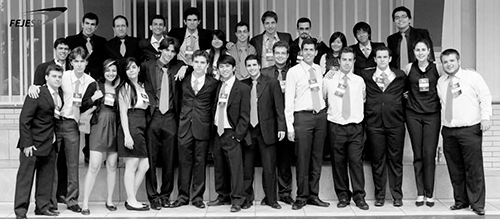
\includegraphics[scale=0.40]{img/alem_da_graduacao/conpec_foto.jpg}
\end{figure}

Para fazer parte da Conpec, fique atento à data da palestra de apresentação do
processo seletivo, que ocorre no início do ano.

Para saber mais sobre a empresa visite o site \url{conpec.com.br} ou tire suas
dúvidas mandando um e-mail para \email{conpec@conpec.com.br}.
